\section{Introduction}
\begin{figure}[htb]
    \centering
    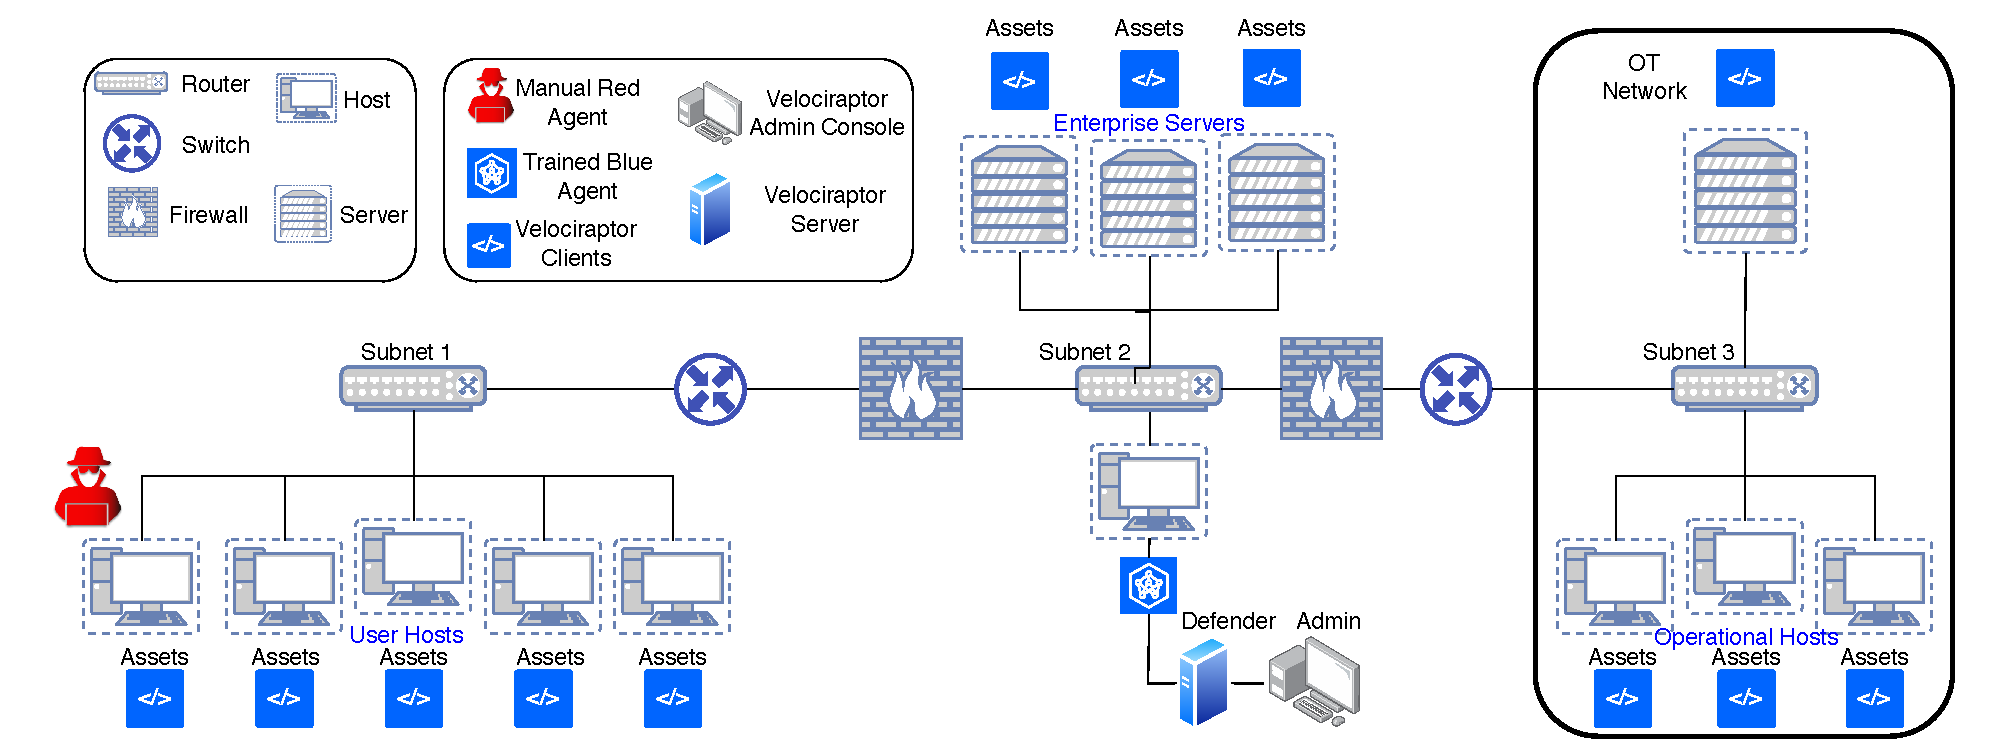
\includegraphics[width=\linewidth,trim={0cm 0cm 0cm 0cm}, clip]{Figures/cage2.pdf}
    \caption{Schematic of the enterprise CAGE-2 network topology with embedded OT network.}
    \label{fig:Enterprise_Network}
\end{figure}
Operational Technology (OT) networks are critical infrastructure systems responsible for controlling physical processes in industries such as manufacturing, energy, transportation, and utilities \cite{negi2024towards} . These networks integrate hardware and software systems, including Supervisory Control and Data Acquisition (SCADA), Programmable Logic Controllers (PLCs), and Distributed Control Systems (DCS), to ensure the smooth operation of industrial machinery and processes. However, with the convergence of OT and Information Technology (IT) systems with increased digitalization and Industry 4.0 initiatives, OT networks have become a prime target for Cyber threats in recent time \cite{knapp2024industrial} \cite{zaid2024emerging}. Unlike traditional IT systems, OT networks face unique cybersecurity challenges due to their legacy systems, real-time operational requirements, and the high economic loss incurred during its downtime or failure. Cybersecurity in OT networks, therefore, focuses on safeguarding critical infrastructure from threats such as malware, ransomware, and state-sponsored attacks, ensuring the continuity, safety, and reliability of essential services.
Attackers target the OT-networks through methods like social engineering, exploiting vulnerabilities in IT components, malware injection, supply chain attacks, and insecure remote access, with spear phishing and the Stuxnet worm as notable examples \cite{stojanovic2020apt}.
These breaches not only compromise sensitive OT systems but also result in significant financial losses, as highlighted in IBM's report \cite{IBM}.
%indicating the loss of millions of dollars per data breach.
%average cost of a data breach at \$4.88 million—a 10\% hike from the previous year—and the Colonial Pipeline ransomware attack, which caused a direct ransom payment of \$4.4 million and significant disruptions.
Moreover, the report also highlights the steep costs associated with downtime in OT,
%(\textasciitilde\$260K/hr.),
emphasizing the critical need for robust OT cybersecurity to prevent such expensive and operationally disruptive incidents. Manual efforts for cybersecurity are time-consuming and error-prone, which necessitates the use of automated cyber agents. However, before deploying these cyber agents must be thoroughly evaluated on their performance because the behavior of the agents could be very different in emulation (that mirrors the real-world use-case) as opposed to in pure network simulation (where these agents are typically trained). This requires a general-purpose, configurable testbed to evaluate cyber agents for the OT networks. Such testbeds are currently lacking.

In this paper, we describe a highly configurable emulation testbed for evaluating cyber agents in the OT networks.
%To curb this threat to the industries, {cybersecurity-agents} or cyber-agents are deployed within the network with diverse objectives.
Our testbed enables realistic evaluation of these cyber agents, thereby bypassing the expensive and rather potentially dangerous real world testing. The proposed emulation environment, hosted on openstack, can be integrated as a subnet of a larger network topology and in its present form, also provides to the users, a programmable interface that is vulnerable to attack. The OT use cases deployed using this testbed, consists of power grid (utility) and chemical plant (industry) environments, whose controllers rely on their respective OT networks for information exchange and control. The visualization of the plant operations along with the information using SCADA, helps users analyze the state of the plant at any time, thereby understanding the impact of an action taken by the agent on the OT network. In addition, we showcase the application of these features within the proposed testbed through the execution of basic network and host attacks, and we observe the ensuing impact on the electrical grid and chemical processing facilities.


The rest of this paper is organized as follows - Section \ref{sec:related} details related work by reviewing the characteristics of existing testbeds and identifies the basic requirements for the testbed.
%states the characteristics of various testbeds we have identified as a potential {cyber-agent} testbed also highlighting some of the requirements a testbed offers.
Section \ref{sec:architecture} describes the overall architecture of our testbed, its design and integration methods. Section \ref{sec:casestudy} presents two case studies covering the attacks on power grid and chemical plant environments and underlines
%discusses the case study using attacks underlining
the limitations that we have identified. Section \ref{sec:conclusion} presents potential future extensions and concluding remarks.


